\lab{Spectral 2: A Pseudospectral method for periodic functions}{Spectral 2: A Pseudospectral method for periodic functions}
\label{lab:pseudospectral2}
\labdependencies{SpectralMethod1}

\objective{
We look at a pseudospectral method with a Fourier basis, and numerically solve two PDEs using a pseudospectral discretization in space and a Runge-Kutta integration scheme in time.  }

Let $f$ be a periodic function on $[0,2\pi]$.
Let $x_1,\ldots,x_N$ be $N$ evenly spaced grid points on $[0,2\pi]$.
Since $f$ is periodic on $[0,2\pi]$, we can ignore the grid point $x_N = 2\pi$.
We will further assume that $N$ is even; similar formulas can be derived for $N$ odd.
Let $h = 2\pi/N$; then $\{x_0,\ldots,x_{N-1}\} = \{0,h,2h,\ldots,2\pi-h\}$.  

The discrete Fourier transform (DFT) of $f$, denoted by $\hat{f}$ or $\mathcal{F}(f)$, is given by
\[
\hat{f}(k) = h \sum_{j=0}^{N-1} e^{-ikx_j}f(x_j) \quad \text{ where } k = -N/2+1, \ldots,0,1,\ldots, N/2.
\]
The inverse DFT is then given by
\begin{align}
\begin{split}
f(x_j) &= \frac{1}{2\pi}\sum_{k=-N/2}^{N/2}\frac{e^{ikx_j}}{c_k}\hat{f}(k), \quad j = 0,\ldots, N-1,
\end{split}\label{inverse_dft}
\end{align}
where
\begin{align}
	c_k = \begin{cases} 2 & \text{if }k = -N/2 \text{ or }k = N/2, \\ 1 &  \text{otherwise.}
\end{cases}
\end{align}
The inverse DFT can then be used to define a natural interpolant (sometimes called a band-limited interpolant) by evaluating (\ref{inverse_dft}) at any $x$ rather than $x_j$:
\begin{align}
p(x) = \frac{1}{2\pi}\sum_{k=-N/2}^{N/2} e^{ikx}\hat{f}(k). \label{interpolant}
\end{align}
The interpolant for $f'$ is then given by 
\begin{align}
p'(x) = \frac{1}{2\pi}\sum_{k=-N/2+1}^{N/2-1} ike^{ikx}\hat{f}(k). \label{spectral2:deriv}
\end{align}

Consider the function $u(x) = \sin^2 (x) \cos(x) +e^{2\sin(x+1)}$. 
Using \eqref{spectral2:deriv}, the derivative $u'$ may be approximated with the following code. 
\footnote{See \textit{Spectral Methods in MATLAB} by Lloyd N. Trefethen.
Another good reference is \textit{Chebyshev and Fourier Spectral Methods} by John P. Boyd.}
We note that although we only approximate $u'$ at the Fourier grid points, \eqref{spectral2:deriv} provides an analytic approximation of $u'$ in the form of a trigonometric polynomial.

\begin{lstlisting}
import numpy as np
from scipy.fftpack import fft, ifft
import matplotlib.pyplot as plt

N=24
x1 = (2.*np.pi/N)*np.arange(1,N+1)
f = np.sin(x1)**2.*np.cos(x1) + np.exp(2.*np.sin(x1+1))

# This array is reordered in Python to
# accomodate the ordering inside the fft function in scipy.
k = np.concatenate(( np.arange(0,N/2) ,
					 np.array([0])	, # Because hat{f}'(k) at k = N/2 is zero.
					 np.arange(-N/2+1,0,1)	))

# Approximates the derivative using the pseudospectral method
f_hat = fft(f)
fp_hat = ((1j*k)*f_hat)
fp = np.real(ifft(fp_hat))

# Calculates the derivative analytically
x2 = np.linspace(0,2*np.pi,200)
derivative = (2.*np.sin(x2)*np.cos(x2)**2. - 
				np.sin(x2)**3. + 
				2*np.cos(x2+1)*np.exp(2*np.sin(x2+1))
				)

plt.plot(x2,derivative,'-k',linewidth=2.)
plt.plot(x1,fp,'*b')
plt.savefig('spectral2_derivative.pdf')
plt.show()
\end{lstlisting}

\begin{figure}[H]
\centering
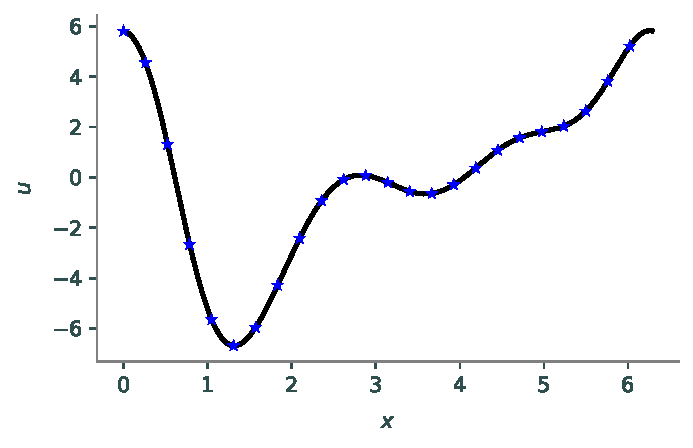
\includegraphics[width=\textwidth]{figures/spectral2_derivative_example.pdf}
\caption{The derivative of $u(x) = \sin^2 (x) \cos(x) +e^{2\sin(x+1)}$.}
\label{fig:spectral:spectral2_derivative}
\end{figure}

\begin{problem}
Consider again the function $u(x) = \sin^2 (x) \cos(x) +e^{2\sin(x+1)}$.
Create a function that approximates $\frac{1}{2}u''-u'$ on the Fourier grid points for $N=24$.	
\end{problem}

\section*{The advection equation}
Recall that the advection equation is given by
\begin{align}
&{ }u_t + cu_x = 0
\end{align}
where $c$ is the speed of the wave (the wave travels to the right for $c > 0$).
We will consider the solution of the advection equation on the domain $[0,2\pi]$ and assume periodic boundary conditions.

A common method for solving time-dependent PDEs is called the \textit{method of lines}.
To apply the method of lines to our problem, we use our Fourier grid points in $[0,2\pi]$: given an even $N$, let $h = 2\pi/N$, so that $\{x_0,\ldots,x_{N-1}\} = \{0,h,2h,\ldots,2\pi-h\}$.
By using these grid points we obtain the collection of equations
\begin{align}
&{ }u_t(x_j,t) + cu_x(x_j,t) = 0, \quad t >0, \quad j = 0, \ldots N-1. \label{spectral2:method_oflines}
\end{align}

Let $U(t)$ be the vector-valued function given by $U(t) = (u(x_j,t))_{j=0}^{N-1}$.
Let $\mathcal{F}(U)(t)$ denote the discrete Fourier transform of $u(x,t)$ (in space), so that 
\[
\mathcal{F}(U)(t) = (\hat{u}(k,t))_{k=-N/2+1}^{N/2}.
\]
Define $\mathcal{F}^{-1}$ similarly.
Using the pseudospectral approximation in space leads to the system of ODEs
\begin{align}
	U_t +  \vec{c}\mathcal{F}^{-1}\left(i\vec{k}\mathcal{F}(U) \right) = 0
\end{align}
where $\vec{k}$ is a vector, and $\vec{k}\mathcal{F}(U) $ denotes element-wise multiplication. 
Similarly $\vec{c}$ could also be a vector, if the wave speed $c$ is allowed to vary. We can then use an ODE solver for the time derivative and the pseudospectral method for spatial derivatives.

\begin{problem}
Using \li{solve_ivp}, solve the initial value problem 
\begin{align}
	u_t +c(x) u_x = 0,
\end{align}
where $c(x) = 0.2 + \sin^2(x-1)$, and $u(x,t=0) = e^{-100(x-1)^2}.$ 
Plot your numerical solution from $t = 0$ to $t = 8$ over 250 time steps and 200 $x$ steps. 
Note that the initial data is nearly zero near $x = 0$ and $2 \pi$, and so we can use the pseudospectral method.\footnote{This problem is solved in \textit{Spectral Methods in MATLAB} using a leapfrog discretization in time. } 
\label{spectral2:advection_equation}
Use the following code to help graph. The solution can be seen in Figure \ref{fig:spectral:spectral2_advection}.
\begin{lstlisting}
t_steps = 250    # Time steps
x_steps = 200     # x steps

'''
Your code here to set things up
'''

sol = # use solve_ivp

X,Y = np.meshgrid(x_domain, t_domain)
fig = plt.figure()
ax = fig.add_subplot(111, projection="3d")
surf = ax.plot_surface(X,Y,np.transpose(sol.y),cmap='coolwarm')
ax.set_zlim(0,3)
ax.view_init(elev=40, azim=280, roll=0)
ax.set_xlabel(r'$x$')
ax.set_ylabel(r'$T$')
ax.set_zlabel(r'$z$')
ax.set_box_aspect(aspect=None, zoom=0.8)
plt.show()
\end{lstlisting}
\end{problem}

\begin{figure}[H]
\centering
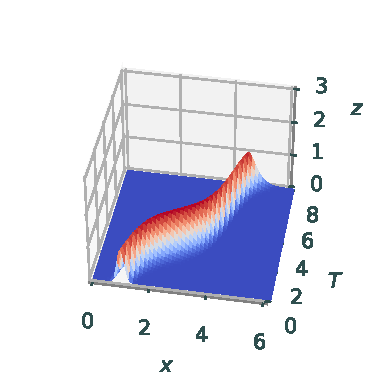
\includegraphics[width=\textwidth]{figures/variable_speed_advection.pdf}
\caption{The solution of the variable speed advection equation; see Problem \ref{spectral2:advection_equation}.}
\label{fig:spectral:spectral2_advection}
\end{figure}

\section*{The wave equation}
We can use the pseudospectral method to solve higher-order PDEs as well. A common example of a second-order hyperbolic PDE is the wave equation, which is often used in physics. The wave equation is given by

\begin{align*}
&{ }u_{tt} - cu_{xx} = 0,
\end{align*}
where $c$ is the wave speed. Unlike the advection equation, waves that encounter mediums of different wave speeds will reflect part of the wave back. We will see this in Problem \ref{spectral2:wave_equation}. First, we must change this second-order method-of-lines ODE equation into a first-order equation.
Using the \textit{method of lines}, the wave equation can be written as a system of first-order ODEs,

\begin{align}
\frac{\partial}{\partial t} \begin{bmatrix}
u\\
u_t \\
\end{bmatrix} &= 
\begin{bmatrix}
u_t\\
cu_{xx}
\end{bmatrix}.
\end{align}
We can then use an ODE solver, such as \li{solve_ivp} to solve for the time derivatives, while we use the spectral method for the spatial derivatives.

\begin{problem}
Using \li{solve_ivp}, solve the initial value problem 
\begin{align}
	u_{tt} -c(x) u_{xx} = 0,
\end{align}
where 
\begin{align*}
c(x)=
\begin{cases}
  4  & 0\leq x < \pi \\
  1  & \pi \leq x < 2\pi
\end{cases},
\end{align*}
with $u(x,t=0) = 0.2e^{(-10(x-5)^2)}$  and $u_t(x,t=0) = -4(x-5)e^{(-10(x-5)^2)}$.
Plot your numerical solution from $t = 0$ to $t = 3$ over 150 time steps and 100 $x$ steps. 
As in the previous problem, the initial data is nearly zero near $x = 0$ and $2 \pi$, and so we can use the pseudospectral method (the solution is approximately periodic because the boundaries both stay near zero).
Use the code provided in the previous problem (but with different numbers of steps in the $x$ and $t$ directions) to help with plotting. The solution can be seen in Figure \ref{fig:spectral:spectral2_wave}. Note that the wave speeds up at the barrier, and some of it is reflected.

Hints: The initial conditions for \li{solve_ivp} need to be in a one-dimensional array. Concatenate the initial conditions into a single $(100+100)\times1$ array to start \li{solve_ivp}. You will need to make corresponding changes in the RHS derivative function (the first parameter of \li{solve_ivp}) by returning a $(100+100)\times1$ array, where the first $100$ elements are the derivative $\frac{\partial}{\partial t}u$, and the second $100$ elements are the derivative $\frac{\partial}{\partial t}u_t$.
\label{spectral2:wave_equation}
\end{problem}

\begin{figure}[H]
\centering
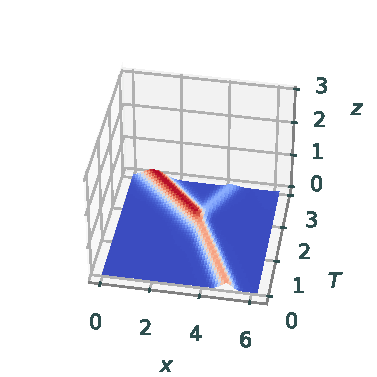
\includegraphics[width=\textwidth]{figures/wave_equation_barrier.pdf}
\caption{The solution of the wave equation for a pulse hitting a barrier at $x=\pi$; see Problem \ref{spectral2:wave_equation}.}
\label{fig:spectral:spectral2_wave}
\end{figure}

